% !TeX spellcheck = en_US
\documentclass{article}

\usepackage[utf8]{inputenc}

\title{
	\textbf{HPC Shallow Water project : Theoretical Analysis}
	\\ [2.0cm]
	}
\author
{Antoine Hoffmann\\
	Parallel and High Performance Computing MATH-454, EPFL\\
	\normalsize{E-mail:  antoine.hoffmann@epfl.ch}\\
}
\date{\today}


\usepackage{graphicx, setspace, booktabs}
\usepackage[left=2cm,right=2cm,top=2cm,bottom=2cm]{geometry}
%\usepackage[myheadings]{fullpage}
\usepackage{fancyhdr}
\usepackage{lastpage}

\pagestyle{fancy}
\fancyhf{}
\setlength\headheight{15pt}
\fancyhead[L]{PHPC project}
\fancyhead[R]{Antoine Hoffmann}
\fancyfoot[R]{Page \thepage\ of \pageref{LastPage}}

\usepackage{algorithm}
\usepackage[noend]{algpseudocode}
\usepackage{amsmath}
\usepackage{amssymb}
%\usepackage{mathtools}
%\usepackage{amsfonts}
%\usepackage{subcaption}

\newcommand{\omegacoeff}{c^{\Omega}}
\newcommand{\phicoeff}{c^{\phi}}
\newcommand{\Rho}{\mathrm{P}}
\newcommand{\spline}{\Lambda^s}

\bibliographystyle{plain}

%%======================================================================================================%%
%%======================================================================================================%%
\begin{document}
\maketitle
\section{Introduction}
This project consist to parallelize a given finite volume solver \textsc{Matlab} code which simulates the propagation of a Tsunami on the scale of an island in the shallow water modeling framework.
\section{Presentation of the sequential C++ code}
\subsection{Sequential Algorithm}
The \textsc{Matlab} code has been firstly translated into a C++ sequential code. The main work consisted mainly in a structural reorganization of the algorithm by defining a collection of C++ functions. Those functions where written in a second C++ file linked to the main program with a hierarchical makefile in view to increase the readability and analysis of performance. The algorithm and the finite volume solver did not need to be deeply changed and one can read a pseudo code presentation of the sequential C++ implementation at Algorithm \ref{alg:sequ}.\\
\begin{algorithm}
	\caption{Sequential C++ Finite Volume Solver}\label{alg:sequ}
\begin{algorithmic}
	\State $n_x =$ 1D number of grid cells on one side of the domain
	\State $N =$ Total number of grid cells
	\State $dx =$ Grid spacening in [km]
	\State Allocating $(H,HU,HV,Z_{dx},Z_{dy},H_t,HU_t,HV_t)$ \Comment{Memory allocation}
	\State $(Z_{dx}, Z_{dy})	\Leftarrow$ Topology data file \Comment{Load gradients of the topology from binary data file}
	\State $(H,HU,HV)\Leftarrow$ Initial state data file  \Comment{Load initial state of the height and the velocities of the water}
	\While{$T < T_{\text{end}}$} \Comment{Simulating until a given time $T_{\text{end}}$ }
	\State $dt \Leftarrow$ new\_dt$(H,HU,HV,dx,N)$\Comment{Updating $dt$ from finite volume scheme}
	\If{$T+dt > T_{\text{end}}$}
	\State $dt \Leftarrow T_{\text{end}}-T$\Comment{To stop exactly at $T_{\text{end}}$}
	\EndIf
	\State $(H_t,HU_t,HV_t)\Leftarrow (H,HU,HV)$\Comment{Copy current state to temporary variables}
	\State $(H_t,HU_t,HV_t)\Leftarrow$ enforce\_BC($H_t,HU_t,HV_t,dx$)\Comment{Enforce boundary conditions}
	\State $(H,HU,HV)\Leftarrow$ FV\_time\_step$(Z_{dx},Z_{dy},H_t,HU_t,HV_t,dt,nx)$\Comment{Perform one time step of finite volume scheme}
	\State $(H,HU,HV)\Leftarrow$ impose\_tolerances$(H,HU,HV)$
	\State $T\Leftarrow T+dt$
	\EndWhile
	\State Save solution to disk
	\State Free memory space
\end{algorithmic}
\end{algorithm}
\subsection{Validation}
Some data are also taken from the C++ code such as the final state of the water level and an history of the time step evolution during the simulation. Those two results were used to verify the correctness of the C++ code. Figure \ref{fig:dt_comparison_sequential} and Figure \ref{fig:matlab_sequCpp_error_solution} confirm that the sequential C++ code is working correctly with a negligible error in comparison to the real values.\\
\begin{figure}[!h]
\centering
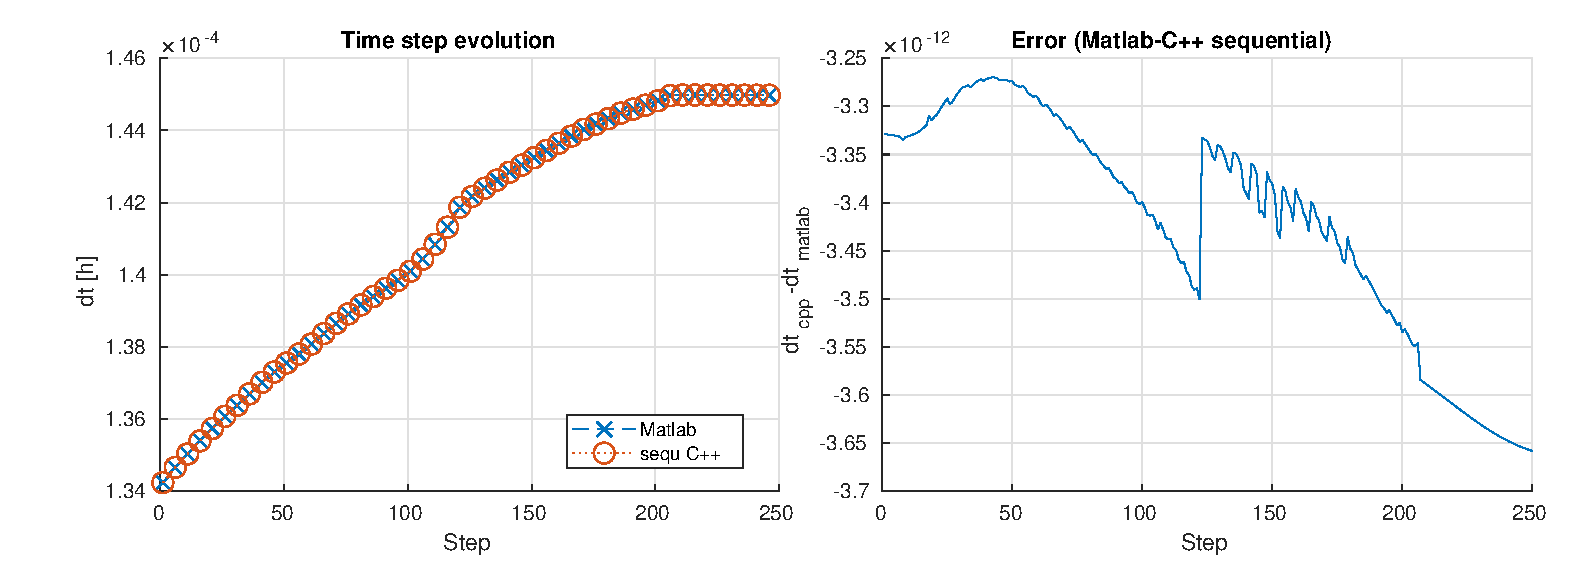
\includegraphics[width=0.9\linewidth]{../figures/dt_comparison_sequential}
\caption{Comparison between the tracking of the time step in the Matlab and C++ sequential codes.}
\label{fig:dt_comparison_sequential}
\end{figure}
\begin{figure}[h!]
\centering
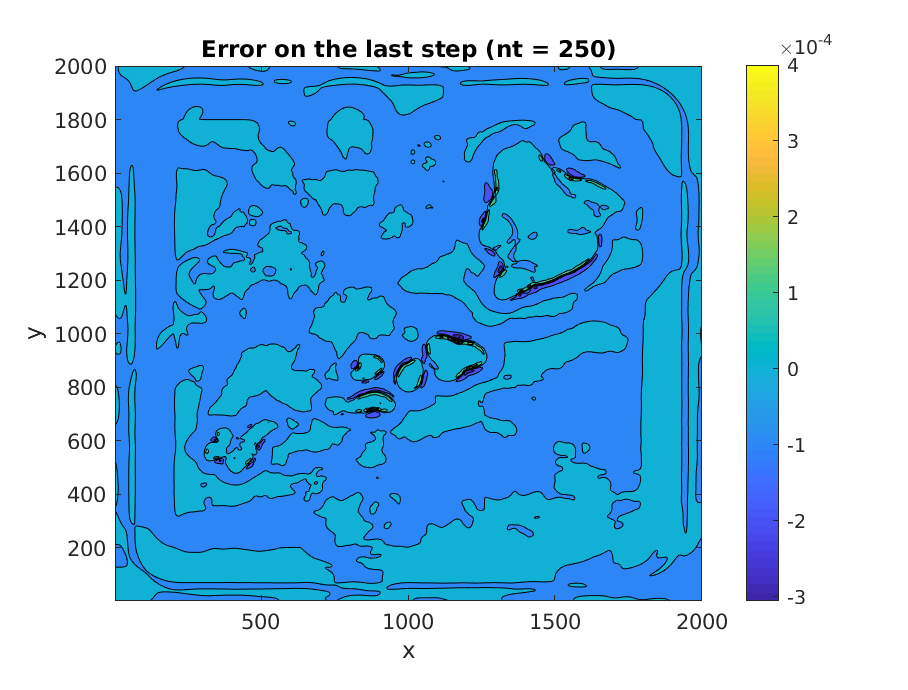
\includegraphics[width=0.7\linewidth]{../figures/matlab_sequCpp_error_solution}
\caption{Error between the last step of the \textsc{Matlab} code and sequential C++ one.}
\label{fig:matlab_sequCpp_error_solution}
\end{figure}
\subsection{Performance comparison}
Even if one could not expect an improvement in performance as great as the future parallelization of the algorithm, it can be interesting to figure out if the C++ language version performs already better the sequential algorithm than the \textsc{Matlab} version. The performances in computational time has been measured through six independent launch of \texttt{compute.m} and \texttt{compute.cpp}. These measurement are reported on Figure \ref{fig:perform_comparison_sequ} where one can observe a $\approx 250\%$ increase of the performance just by transferring the solver from \textsc{Matlab} to C++. Of course the performance of the C++ code is related to the compilation process did with the most aggressive optimization option (\texttt{-Ofast}). The least optimized compilation (\texttt{-O0}) shows extremely reduced performances and take more than $300$ seconds to run.
\begin{figure}[h!]
	\centering
	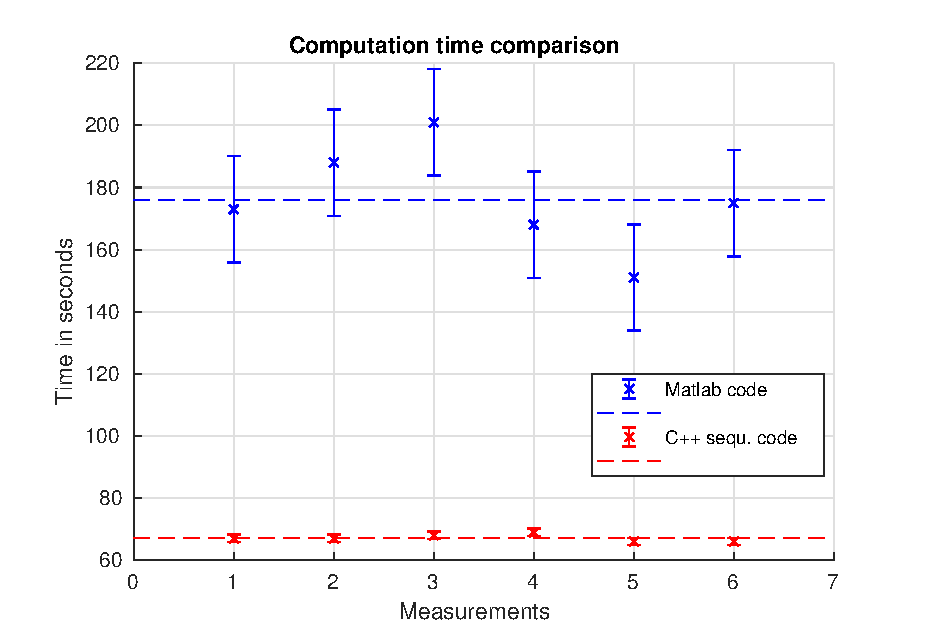
\includegraphics[width=0.7\linewidth]{../figures/perform_comparison_sequ}
	\caption{Performance comparison between \textsc{Matlab} and sequential C++ code for $250$ iterations and \texttt{g++ -Ofast} compilation option on an Intel(R) Core(TM) i7-6700HQ CPU @ 2.60GHz.}
	\label{fig:perform_comparison_sequ}
\end{figure}
\subsection{Computing time analysis}
Before starting the parallelization of our sequential code, it is important to perform a profiling of the computational cost of each steps in the Algorithm \ref{alg:sequ}. The Table \ref{tab:manual_sequ_profiling} presents the computational times (expressed in ticks) taken by the main process of our sequential code and the percentage it represents w.r.t. the global computational time. One can notice that the most costly part of the algorithm is to compute the steps of the finite volume explicit scheme. Keeping this in mind, a parallelization of the function \texttt{FV\_time\_step} must be the priority.
\begin{table}[h!]
	\centering
\begin{tabular}{l|c|r}
	Step & Comp. Time [ms] & Share of total time \\
	\hline 
	Variable Initialization 	& $0.0432	\pm	0.0447$ & $<0.0001\%$ \\ 
	Initial state loading 		& $57.021	\pm	3.771$ 	& $0.0880	\pm	0.0073\%$ \\ 
	\texttt{new\_dt} 			& $3532.6	\pm	79.5$ 	& $5.4466	\pm	0.0741\%$ \\ 
	Copy to temporary variables & $2870.8	\pm	51.017$ & $4.4271	\pm	0.0874\%$ \\ 
	\texttt{enfore\_BC} 		& $34.669	\pm	1.9657$ & $0.0534	\pm	0.0017\%$ \\ 
	\texttt{FV\_time\_step} 	& $57608	\pm	1551.2$ & $88.8071	\pm	0.1638\%$ \\ 
	\texttt{impose\_tolerances} & $729.33	\pm	21.124$ & $1.1245	\pm	0.0239\%$ \\ 
	Save output 				& $25.334	\pm	1.4030$	& $0.0390	\pm 0.0014\%$ \\ 
	Free memory space 			& $9.1721	\pm	0.3275$ & $0.0141	\pm 0.0002\%$\\
	\hline
\end{tabular} 
\caption{Results for $10$ manual profiling of the sequential C++ code for $250$ step.}
\label{tab:manual_sequ_profiling}
\end{table}

\section{Parallelism Preview with CUDA}
The GPU programming language CUDA has been chosen to implement a parallel version of the C++ sequential code.\\The parallelization of the main \texttt{while} loop of Algorithm \ref{alg:sequ} can obviously not be parallelized since it needs the results of the previous iteration at each steps. It is however not the case for the functions called inside the loop, i.e. \texttt{new\_dt}, \texttt{enforce\_BC}, \texttt{FV\_time\_step} and \texttt{impose\_tolerances}. 
\subsection{Parallelization of \texttt{FV\_time\_step}} 
As demonstrated on Table \ref{tab:manual_sequ_profiling}, the \texttt{FV\_time\_step} function has the greatest potential of performance increase.\\ Since the treated variables are two dimensional arrays, the most natural way to parallelize this function is to divide the grid in to $N_b$ regions. Each region will be treated by one block containing $N_t=N/N_b$ threads.
However the process updates the variables $H,HU$ and $HV$ by performing a computation similar to a second degree derivative finite difference scheme, thus some data must be transfered between the blocks on their borders.
\bibliographystyle{ieeetr}

\end{document}
